% Generated by ArticleSignalDiagrams. Opaque vector fills only.
\documentclass[10pt,tikz,border=5pt]{standalone}
\usepackage{lmodern}
\usetikzlibrary{fit}
\begin{document}
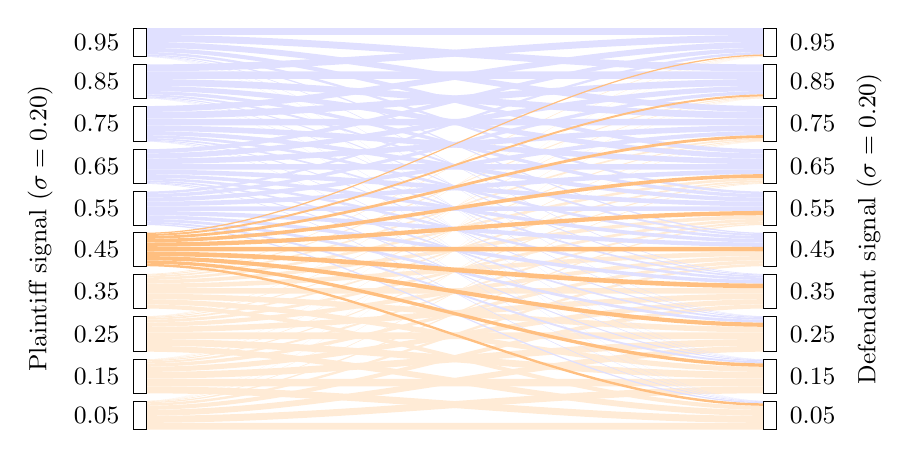
\begin{tikzpicture}[x=1cm,y=1cm,font=\small]\path[fill=orange!16!white,draw=none] (3.3,-5.1) .. controls (6,-5.1) and (8.6,-5.1) .. (11.3,-5.1) -- (11.3,-5.013686) .. controls (8.6,-5.013686) and (6,-5.013686) .. (3.3,-5.013686) -- cycle;
\path[fill=orange!16!white,draw=none] (3.3,-5.013686) .. controls (6,-5.013686) and (8.6,-4.637713) .. (11.3,-4.637713) -- (11.3,-4.549059) .. controls (8.6,-4.549059) and (6,-4.925033) .. (3.3,-4.925033) -- cycle;
\path[fill=orange!16!white,draw=none] (3.3,-4.925033) .. controls (6,-4.925033) and (8.6,-4.109199) .. (11.3,-4.109199) -- (11.3,-4.034411) .. controls (8.6,-4.034411) and (6,-4.850245) .. (3.3,-4.850245) -- cycle;
\path[fill=orange!16!white,draw=none] (3.3,-4.850245) .. controls (6,-4.850245) and (8.6,-3.560821) .. (11.3,-3.560821) -- (11.3,-3.508204) .. controls (8.6,-3.508204) and (6,-4.797628) .. (3.3,-4.797628) -- cycle;
\path[fill=orange!16!white,draw=none] (3.3,-4.797628) .. controls (6,-4.797628) and (8.6,-3.02315) .. (11.3,-3.02315) -- (11.3,-2.991698) .. controls (8.6,-2.991698) and (6,-4.766176) .. (3.3,-4.766176) -- cycle;
\path[fill=orange!16!white,draw=none] (3.3,-4.766176) .. controls (6,-4.766176) and (8.6,-2.5) .. (11.3,-2.5) -- (11.3,-2.483692) .. controls (8.6,-2.483692) and (6,-4.749868) .. (3.3,-4.749868) -- cycle;
\path[fill=orange!16!white,draw=none] (3.3,-4.749868) .. controls (6,-4.749868) and (8.6,-1.97685) .. (11.3,-1.97685) -- (11.3,-1.969364) .. controls (8.6,-1.969364) and (6,-4.742381) .. (3.3,-4.742381) -- cycle;
\path[fill=orange!16!white,draw=none] (3.3,-4.742381) .. controls (6,-4.742381) and (8.6,-1.439179) .. (11.3,-1.439179) -- (11.3,-1.436082) .. controls (8.6,-1.436082) and (6,-4.739285) .. (3.3,-4.739285) -- cycle;
\path[fill=orange!16!white,draw=none] (3.3,-4.739285) .. controls (6,-4.739285) and (8.6,-0.890801) .. (11.3,-0.890801) -- (11.3,-0.889633) .. controls (8.6,-0.889633) and (6,-4.738117) .. (3.3,-4.738117) -- cycle;
\path[fill=orange!16!white,draw=none] (3.3,-4.738117) .. controls (6,-4.738117) and (8.6,-0.362287) .. (11.3,-0.362287) -- (11.3,-0.361883) .. controls (8.6,-0.361883) and (6,-4.737713) .. (3.3,-4.737713) -- cycle;
\path[fill=orange!16!white,draw=none] (3.3,-4.637713) .. controls (6,-4.637713) and (8.6,-5.013686) .. (11.3,-5.013686) -- (11.3,-4.925033) .. controls (8.6,-4.925033) and (6,-4.549059) .. (3.3,-4.549059) -- cycle;
\path[fill=orange!16!white,draw=none] (3.3,-4.549059) .. controls (6,-4.549059) and (8.6,-4.549059) .. (11.3,-4.549059) -- (11.3,-4.453522) .. controls (8.6,-4.453522) and (6,-4.453522) .. (3.3,-4.453522) -- cycle;
\path[fill=orange!16!white,draw=none] (3.3,-4.453522) .. controls (6,-4.453522) and (8.6,-4.034411) .. (11.3,-4.034411) -- (11.3,-3.948547) .. controls (8.6,-3.948547) and (6,-4.367658) .. (3.3,-4.367658) -- cycle;
\path[fill=orange!16!white,draw=none] (3.3,-4.367658) .. controls (6,-4.367658) and (8.6,-3.508204) .. (11.3,-3.508204) -- (11.3,-3.442636) .. controls (8.6,-3.442636) and (6,-4.30209) .. (3.3,-4.30209) -- cycle;
\path[fill=orange!16!white,draw=none] (3.3,-4.30209) .. controls (6,-4.30209) and (8.6,-2.991698) .. (11.3,-2.991698) -- (11.3,-2.948266) .. controls (8.6,-2.948266) and (6,-4.258657) .. (3.3,-4.258657) -- cycle;
\path[fill=orange!16!white,draw=none] (3.3,-4.258657) .. controls (6,-4.258657) and (8.6,-2.483692) .. (11.3,-2.483692) -- (11.3,-2.458219) .. controls (8.6,-2.458219) and (6,-4.233184) .. (3.3,-4.233184) -- cycle;
\path[fill=orange!16!white,draw=none] (3.3,-4.233184) .. controls (6,-4.233184) and (8.6,-1.969364) .. (11.3,-1.969364) -- (11.3,-1.955903) .. controls (8.6,-1.955903) and (6,-4.219723) .. (3.3,-4.219723) -- cycle;
\path[fill=orange!16!white,draw=none] (3.3,-4.219723) .. controls (6,-4.219723) and (8.6,-1.436082) .. (11.3,-1.436082) -- (11.3,-1.429596) .. controls (8.6,-1.429596) and (6,-4.213237) .. (3.3,-4.213237) -- cycle;
\path[fill=orange!16!white,draw=none] (3.3,-4.213237) .. controls (6,-4.213237) and (8.6,-0.889633) .. (11.3,-0.889633) -- (11.3,-0.886763) .. controls (8.6,-0.886763) and (6,-4.210367) .. (3.3,-4.210367) -- cycle;
\path[fill=orange!16!white,draw=none] (3.3,-4.210367) .. controls (6,-4.210367) and (8.6,-0.361883) .. (11.3,-0.361883) -- (11.3,-0.360715) .. controls (8.6,-0.360715) and (6,-4.209199) .. (3.3,-4.209199) -- cycle;
\path[fill=orange!16!white,draw=none] (3.3,-4.109199) .. controls (6,-4.109199) and (8.6,-4.925033) .. (11.3,-4.925033) -- (11.3,-4.850245) .. controls (8.6,-4.850245) and (6,-4.034411) .. (3.3,-4.034411) -- cycle;
\path[fill=orange!16!white,draw=none] (3.3,-4.034411) .. controls (6,-4.034411) and (8.6,-4.453522) .. (11.3,-4.453522) -- (11.3,-4.367658) .. controls (8.6,-4.367658) and (6,-3.948547) .. (3.3,-3.948547) -- cycle;
\path[fill=orange!16!white,draw=none] (3.3,-3.948547) .. controls (6,-3.948547) and (8.6,-3.948547) .. (11.3,-3.948547) -- (11.3,-3.864786) .. controls (8.6,-3.864786) and (6,-3.864786) .. (3.3,-3.864786) -- cycle;
\path[fill=orange!16!white,draw=none] (3.3,-3.864786) .. controls (6,-3.864786) and (8.6,-3.442636) .. (11.3,-3.442636) -- (11.3,-3.371758) .. controls (8.6,-3.371758) and (6,-3.793908) .. (3.3,-3.793908) -- cycle;
\path[fill=orange!16!white,draw=none] (3.3,-3.793908) .. controls (6,-3.793908) and (8.6,-2.948266) .. (11.3,-2.948266) -- (11.3,-2.89516) .. controls (8.6,-2.89516) and (6,-3.740802) .. (3.3,-3.740802) -- cycle;
\path[fill=orange!16!white,draw=none] (3.3,-3.740802) .. controls (6,-3.740802) and (8.6,-2.458219) .. (11.3,-2.458219) -- (11.3,-2.422369) .. controls (8.6,-2.422369) and (6,-3.704952) .. (3.3,-3.704952) -- cycle;
\path[fill=orange!16!white,draw=none] (3.3,-3.704952) .. controls (6,-3.704952) and (8.6,-1.955903) .. (11.3,-1.955903) -- (11.3,-1.933831) .. controls (8.6,-1.933831) and (6,-3.68288) .. (3.3,-3.68288) -- cycle;
\path[fill=orange!16!white,draw=none] (3.3,-3.68288) .. controls (6,-3.68288) and (8.6,-1.429596) .. (11.3,-1.429596) -- (11.3,-1.41712) .. controls (8.6,-1.41712) and (6,-3.670404) .. (3.3,-3.670404) -- cycle;
\path[fill=orange!16!white,draw=none] (3.3,-3.670404) .. controls (6,-3.670404) and (8.6,-0.886763) .. (11.3,-0.886763) -- (11.3,-0.880277) .. controls (8.6,-0.880277) and (6,-3.663918) .. (3.3,-3.663918) -- cycle;
\path[fill=orange!16!white,draw=none] (3.3,-3.663918) .. controls (6,-3.663918) and (8.6,-0.360715) .. (11.3,-0.360715) -- (11.3,-0.357619) .. controls (8.6,-0.357619) and (6,-3.660821) .. (3.3,-3.660821) -- cycle;
\path[fill=orange!16!white,draw=none] (3.3,-3.560821) .. controls (6,-3.560821) and (8.6,-4.850245) .. (11.3,-4.850245) -- (11.3,-4.797628) .. controls (8.6,-4.797628) and (6,-3.508204) .. (3.3,-3.508204) -- cycle;
\path[fill=orange!16!white,draw=none] (3.3,-3.508204) .. controls (6,-3.508204) and (8.6,-4.367658) .. (11.3,-4.367658) -- (11.3,-4.30209) .. controls (8.6,-4.30209) and (6,-3.442636) .. (3.3,-3.442636) -- cycle;
\path[fill=orange!16!white,draw=none] (3.3,-3.442636) .. controls (6,-3.442636) and (8.6,-3.864786) .. (11.3,-3.864786) -- (11.3,-3.793908) .. controls (8.6,-3.793908) and (6,-3.371758) .. (3.3,-3.371758) -- cycle;
\path[fill=orange!16!white,draw=none] (3.3,-3.371758) .. controls (6,-3.371758) and (8.6,-3.371758) .. (11.3,-3.371758) -- (11.3,-3.303917) .. controls (8.6,-3.303917) and (6,-3.303917) .. (3.3,-3.303917) -- cycle;
\path[fill=orange!16!white,draw=none] (3.3,-3.303917) .. controls (6,-3.303917) and (8.6,-2.89516) .. (11.3,-2.89516) -- (11.3,-2.836654) .. controls (8.6,-2.836654) and (6,-3.245411) .. (3.3,-3.245411) -- cycle;
\path[fill=orange!16!white,draw=none] (3.3,-3.245411) .. controls (6,-3.245411) and (8.6,-2.422369) .. (11.3,-2.422369) -- (11.3,-2.376353) .. controls (8.6,-2.376353) and (6,-3.199396) .. (3.3,-3.199396) -- cycle;
\path[fill=orange!16!white,draw=none] (3.3,-3.199396) .. controls (6,-3.199396) and (8.6,-1.933831) .. (11.3,-1.933831) -- (11.3,-1.900604) .. controls (8.6,-1.900604) and (6,-3.166169) .. (3.3,-3.166169) -- cycle;
\path[fill=orange!16!white,draw=none] (3.3,-3.166169) .. controls (6,-3.166169) and (8.6,-1.41712) .. (11.3,-1.41712) -- (11.3,-1.395048) .. controls (8.6,-1.395048) and (6,-3.144097) .. (3.3,-3.144097) -- cycle;
\path[fill=orange!16!white,draw=none] (3.3,-3.144097) .. controls (6,-3.144097) and (8.6,-0.880277) .. (11.3,-0.880277) -- (11.3,-0.866816) .. controls (8.6,-0.866816) and (6,-3.130636) .. (3.3,-3.130636) -- cycle;
\path[fill=orange!16!white,draw=none] (3.3,-3.130636) .. controls (6,-3.130636) and (8.6,-0.357619) .. (11.3,-0.357619) -- (11.3,-0.350132) .. controls (8.6,-0.350132) and (6,-3.12315) .. (3.3,-3.12315) -- cycle;
\path[fill=blue!12!white,draw=none] (3.3,-2.5) .. controls (6,-2.5) and (8.6,-4.766176) .. (11.3,-4.766176) -- (11.3,-4.749868) .. controls (8.6,-4.749868) and (6,-2.483692) .. (3.3,-2.483692) -- cycle;
\path[fill=blue!12!white,draw=none] (3.3,-2.483692) .. controls (6,-2.483692) and (8.6,-4.258657) .. (11.3,-4.258657) -- (11.3,-4.233184) .. controls (8.6,-4.233184) and (6,-2.458219) .. (3.3,-2.458219) -- cycle;
\path[fill=blue!12!white,draw=none] (3.3,-2.458219) .. controls (6,-2.458219) and (8.6,-3.740802) .. (11.3,-3.740802) -- (11.3,-3.704952) .. controls (8.6,-3.704952) and (6,-2.422369) .. (3.3,-2.422369) -- cycle;
\path[fill=blue!12!white,draw=none] (3.3,-2.422369) .. controls (6,-2.422369) and (8.6,-3.245411) .. (11.3,-3.245411) -- (11.3,-3.199396) .. controls (8.6,-3.199396) and (6,-2.376353) .. (3.3,-2.376353) -- cycle;
\path[fill=blue!12!white,draw=none] (3.3,-2.376353) .. controls (6,-2.376353) and (8.6,-2.777871) .. (11.3,-2.777871) -- (11.3,-2.723647) .. controls (8.6,-2.723647) and (6,-2.322129) .. (3.3,-2.322129) -- cycle;
\path[fill=blue!12!white,draw=none] (3.3,-2.322129) .. controls (6,-2.322129) and (8.6,-2.322129) .. (11.3,-2.322129) -- (11.3,-2.263346) .. controls (8.6,-2.263346) and (6,-2.263346) .. (3.3,-2.263346) -- cycle;
\path[fill=blue!12!white,draw=none] (3.3,-2.263346) .. controls (6,-2.263346) and (8.6,-1.854589) .. (11.3,-1.854589) -- (11.3,-1.796083) .. controls (8.6,-1.796083) and (6,-2.20484) .. (3.3,-2.20484) -- cycle;
\path[fill=blue!12!white,draw=none] (3.3,-2.20484) .. controls (6,-2.20484) and (8.6,-1.359198) .. (11.3,-1.359198) -- (11.3,-1.306092) .. controls (8.6,-1.306092) and (6,-2.151734) .. (3.3,-2.151734) -- cycle;
\path[fill=blue!12!white,draw=none] (3.3,-2.151734) .. controls (6,-2.151734) and (8.6,-0.841343) .. (11.3,-0.841343) -- (11.3,-0.79791) .. controls (8.6,-0.79791) and (6,-2.108302) .. (3.3,-2.108302) -- cycle;
\path[fill=blue!12!white,draw=none] (3.3,-2.108302) .. controls (6,-2.108302) and (8.6,-0.333824) .. (11.3,-0.333824) -- (11.3,-0.302372) .. controls (8.6,-0.302372) and (6,-2.07685) .. (3.3,-2.07685) -- cycle;
\path[fill=blue!12!white,draw=none] (3.3,-1.97685) .. controls (6,-1.97685) and (8.6,-4.749868) .. (11.3,-4.749868) -- (11.3,-4.742381) .. controls (8.6,-4.742381) and (6,-1.969364) .. (3.3,-1.969364) -- cycle;
\path[fill=blue!12!white,draw=none] (3.3,-1.969364) .. controls (6,-1.969364) and (8.6,-4.233184) .. (11.3,-4.233184) -- (11.3,-4.219723) .. controls (8.6,-4.219723) and (6,-1.955903) .. (3.3,-1.955903) -- cycle;
\path[fill=blue!12!white,draw=none] (3.3,-1.955903) .. controls (6,-1.955903) and (8.6,-3.704952) .. (11.3,-3.704952) -- (11.3,-3.68288) .. controls (8.6,-3.68288) and (6,-1.933831) .. (3.3,-1.933831) -- cycle;
\path[fill=blue!12!white,draw=none] (3.3,-1.933831) .. controls (6,-1.933831) and (8.6,-3.199396) .. (11.3,-3.199396) -- (11.3,-3.166169) .. controls (8.6,-3.166169) and (6,-1.900604) .. (3.3,-1.900604) -- cycle;
\path[fill=blue!12!white,draw=none] (3.3,-1.900604) .. controls (6,-1.900604) and (8.6,-2.723647) .. (11.3,-2.723647) -- (11.3,-2.677631) .. controls (8.6,-2.677631) and (6,-1.854589) .. (3.3,-1.854589) -- cycle;
\path[fill=blue!12!white,draw=none] (3.3,-1.854589) .. controls (6,-1.854589) and (8.6,-2.263346) .. (11.3,-2.263346) -- (11.3,-2.20484) .. controls (8.6,-2.20484) and (6,-1.796083) .. (3.3,-1.796083) -- cycle;
\path[fill=blue!12!white,draw=none] (3.3,-1.796083) .. controls (6,-1.796083) and (8.6,-1.796083) .. (11.3,-1.796083) -- (11.3,-1.728242) .. controls (8.6,-1.728242) and (6,-1.728242) .. (3.3,-1.728242) -- cycle;
\path[fill=blue!12!white,draw=none] (3.3,-1.728242) .. controls (6,-1.728242) and (8.6,-1.306092) .. (11.3,-1.306092) -- (11.3,-1.235214) .. controls (8.6,-1.235214) and (6,-1.657364) .. (3.3,-1.657364) -- cycle;
\path[fill=blue!12!white,draw=none] (3.3,-1.657364) .. controls (6,-1.657364) and (8.6,-0.79791) .. (11.3,-0.79791) -- (11.3,-0.732342) .. controls (8.6,-0.732342) and (6,-1.591796) .. (3.3,-1.591796) -- cycle;
\path[fill=blue!12!white,draw=none] (3.3,-1.591796) .. controls (6,-1.591796) and (8.6,-0.302372) .. (11.3,-0.302372) -- (11.3,-0.249755) .. controls (8.6,-0.249755) and (6,-1.539179) .. (3.3,-1.539179) -- cycle;
\path[fill=blue!12!white,draw=none] (3.3,-1.439179) .. controls (6,-1.439179) and (8.6,-4.742381) .. (11.3,-4.742381) -- (11.3,-4.739285) .. controls (8.6,-4.739285) and (6,-1.436082) .. (3.3,-1.436082) -- cycle;
\path[fill=blue!12!white,draw=none] (3.3,-1.436082) .. controls (6,-1.436082) and (8.6,-4.219723) .. (11.3,-4.219723) -- (11.3,-4.213237) .. controls (8.6,-4.213237) and (6,-1.429596) .. (3.3,-1.429596) -- cycle;
\path[fill=blue!12!white,draw=none] (3.3,-1.429596) .. controls (6,-1.429596) and (8.6,-3.68288) .. (11.3,-3.68288) -- (11.3,-3.670404) .. controls (8.6,-3.670404) and (6,-1.41712) .. (3.3,-1.41712) -- cycle;
\path[fill=blue!12!white,draw=none] (3.3,-1.41712) .. controls (6,-1.41712) and (8.6,-3.166169) .. (11.3,-3.166169) -- (11.3,-3.144097) .. controls (8.6,-3.144097) and (6,-1.395048) .. (3.3,-1.395048) -- cycle;
\path[fill=blue!12!white,draw=none] (3.3,-1.395048) .. controls (6,-1.395048) and (8.6,-2.677631) .. (11.3,-2.677631) -- (11.3,-2.641781) .. controls (8.6,-2.641781) and (6,-1.359198) .. (3.3,-1.359198) -- cycle;
\path[fill=blue!12!white,draw=none] (3.3,-1.359198) .. controls (6,-1.359198) and (8.6,-2.20484) .. (11.3,-2.20484) -- (11.3,-2.151734) .. controls (8.6,-2.151734) and (6,-1.306092) .. (3.3,-1.306092) -- cycle;
\path[fill=blue!12!white,draw=none] (3.3,-1.306092) .. controls (6,-1.306092) and (8.6,-1.728242) .. (11.3,-1.728242) -- (11.3,-1.657364) .. controls (8.6,-1.657364) and (6,-1.235214) .. (3.3,-1.235214) -- cycle;
\path[fill=blue!12!white,draw=none] (3.3,-1.235214) .. controls (6,-1.235214) and (8.6,-1.235214) .. (11.3,-1.235214) -- (11.3,-1.151453) .. controls (8.6,-1.151453) and (6,-1.151453) .. (3.3,-1.151453) -- cycle;
\path[fill=blue!12!white,draw=none] (3.3,-1.151453) .. controls (6,-1.151453) and (8.6,-0.732342) .. (11.3,-0.732342) -- (11.3,-0.646478) .. controls (8.6,-0.646478) and (6,-1.065589) .. (3.3,-1.065589) -- cycle;
\path[fill=blue!12!white,draw=none] (3.3,-1.065589) .. controls (6,-1.065589) and (8.6,-0.249755) .. (11.3,-0.249755) -- (11.3,-0.174967) .. controls (8.6,-0.174967) and (6,-0.990801) .. (3.3,-0.990801) -- cycle;
\path[fill=blue!12!white,draw=none] (3.3,-0.890801) .. controls (6,-0.890801) and (8.6,-4.739285) .. (11.3,-4.739285) -- (11.3,-4.738117) .. controls (8.6,-4.738117) and (6,-0.889633) .. (3.3,-0.889633) -- cycle;
\path[fill=blue!12!white,draw=none] (3.3,-0.889633) .. controls (6,-0.889633) and (8.6,-4.213237) .. (11.3,-4.213237) -- (11.3,-4.210367) .. controls (8.6,-4.210367) and (6,-0.886763) .. (3.3,-0.886763) -- cycle;
\path[fill=blue!12!white,draw=none] (3.3,-0.886763) .. controls (6,-0.886763) and (8.6,-3.670404) .. (11.3,-3.670404) -- (11.3,-3.663918) .. controls (8.6,-3.663918) and (6,-0.880277) .. (3.3,-0.880277) -- cycle;
\path[fill=blue!12!white,draw=none] (3.3,-0.880277) .. controls (6,-0.880277) and (8.6,-3.144097) .. (11.3,-3.144097) -- (11.3,-3.130636) .. controls (8.6,-3.130636) and (6,-0.866816) .. (3.3,-0.866816) -- cycle;
\path[fill=blue!12!white,draw=none] (3.3,-0.866816) .. controls (6,-0.866816) and (8.6,-2.641781) .. (11.3,-2.641781) -- (11.3,-2.616308) .. controls (8.6,-2.616308) and (6,-0.841343) .. (3.3,-0.841343) -- cycle;
\path[fill=blue!12!white,draw=none] (3.3,-0.841343) .. controls (6,-0.841343) and (8.6,-2.151734) .. (11.3,-2.151734) -- (11.3,-2.108302) .. controls (8.6,-2.108302) and (6,-0.79791) .. (3.3,-0.79791) -- cycle;
\path[fill=blue!12!white,draw=none] (3.3,-0.79791) .. controls (6,-0.79791) and (8.6,-1.657364) .. (11.3,-1.657364) -- (11.3,-1.591796) .. controls (8.6,-1.591796) and (6,-0.732342) .. (3.3,-0.732342) -- cycle;
\path[fill=blue!12!white,draw=none] (3.3,-0.732342) .. controls (6,-0.732342) and (8.6,-1.151453) .. (11.3,-1.151453) -- (11.3,-1.065589) .. controls (8.6,-1.065589) and (6,-0.646478) .. (3.3,-0.646478) -- cycle;
\path[fill=blue!12!white,draw=none] (3.3,-0.646478) .. controls (6,-0.646478) and (8.6,-0.646478) .. (11.3,-0.646478) -- (11.3,-0.550941) .. controls (8.6,-0.550941) and (6,-0.550941) .. (3.3,-0.550941) -- cycle;
\path[fill=blue!12!white,draw=none] (3.3,-0.550941) .. controls (6,-0.550941) and (8.6,-0.174967) .. (11.3,-0.174967) -- (11.3,-0.086314) .. controls (8.6,-0.086314) and (6,-0.462287) .. (3.3,-0.462287) -- cycle;
\path[fill=blue!12!white,draw=none] (3.3,-0.362287) .. controls (6,-0.362287) and (8.6,-4.738117) .. (11.3,-4.738117) -- (11.3,-4.737713) .. controls (8.6,-4.737713) and (6,-0.361883) .. (3.3,-0.361883) -- cycle;
\path[fill=blue!12!white,draw=none] (3.3,-0.361883) .. controls (6,-0.361883) and (8.6,-4.210367) .. (11.3,-4.210367) -- (11.3,-4.209199) .. controls (8.6,-4.209199) and (6,-0.360715) .. (3.3,-0.360715) -- cycle;
\path[fill=blue!12!white,draw=none] (3.3,-0.360715) .. controls (6,-0.360715) and (8.6,-3.663918) .. (11.3,-3.663918) -- (11.3,-3.660821) .. controls (8.6,-3.660821) and (6,-0.357619) .. (3.3,-0.357619) -- cycle;
\path[fill=blue!12!white,draw=none] (3.3,-0.357619) .. controls (6,-0.357619) and (8.6,-3.130636) .. (11.3,-3.130636) -- (11.3,-3.12315) .. controls (8.6,-3.12315) and (6,-0.350132) .. (3.3,-0.350132) -- cycle;
\path[fill=blue!12!white,draw=none] (3.3,-0.350132) .. controls (6,-0.350132) and (8.6,-2.616308) .. (11.3,-2.616308) -- (11.3,-2.6) .. controls (8.6,-2.6) and (6,-0.333824) .. (3.3,-0.333824) -- cycle;
\path[fill=blue!12!white,draw=none] (3.3,-0.333824) .. controls (6,-0.333824) and (8.6,-2.108302) .. (11.3,-2.108302) -- (11.3,-2.07685) .. controls (8.6,-2.07685) and (6,-0.302372) .. (3.3,-0.302372) -- cycle;
\path[fill=blue!12!white,draw=none] (3.3,-0.302372) .. controls (6,-0.302372) and (8.6,-1.591796) .. (11.3,-1.591796) -- (11.3,-1.539179) .. controls (8.6,-1.539179) and (6,-0.249755) .. (3.3,-0.249755) -- cycle;
\path[fill=blue!12!white,draw=none] (3.3,-0.249755) .. controls (6,-0.249755) and (8.6,-1.065589) .. (11.3,-1.065589) -- (11.3,-0.990801) .. controls (8.6,-0.990801) and (6,-0.174967) .. (3.3,-0.174967) -- cycle;
\path[fill=blue!12!white,draw=none] (3.3,-0.174967) .. controls (6,-0.174967) and (8.6,-0.550941) .. (11.3,-0.550941) -- (11.3,-0.462287) .. controls (8.6,-0.462287) and (6,-0.086314) .. (3.3,-0.086314) -- cycle;
\path[fill=blue!12!white,draw=none] (3.3,-0.086314) .. controls (6,-0.086314) and (8.6,-0.086314) .. (11.3,-0.086314) -- (11.3,-0) .. controls (8.6,-0) and (6,-0) .. (3.3,-0) -- cycle;
\path[fill=orange!50!white,draw=none] (3.3,-3.02315) .. controls (6,-3.02315) and (8.6,-4.797628) .. (11.3,-4.797628) -- (11.3,-4.766176) .. controls (8.6,-4.766176) and (6,-2.991698) .. (3.3,-2.991698) -- cycle;
\path[fill=orange!50!white,draw=none] (3.3,-2.991698) .. controls (6,-2.991698) and (8.6,-4.30209) .. (11.3,-4.30209) -- (11.3,-4.258657) .. controls (8.6,-4.258657) and (6,-2.948266) .. (3.3,-2.948266) -- cycle;
\path[fill=orange!50!white,draw=none] (3.3,-2.948266) .. controls (6,-2.948266) and (8.6,-3.793908) .. (11.3,-3.793908) -- (11.3,-3.740802) .. controls (8.6,-3.740802) and (6,-2.89516) .. (3.3,-2.89516) -- cycle;
\path[fill=orange!50!white,draw=none] (3.3,-2.89516) .. controls (6,-2.89516) and (8.6,-3.303917) .. (11.3,-3.303917) -- (11.3,-3.245411) .. controls (8.6,-3.245411) and (6,-2.836654) .. (3.3,-2.836654) -- cycle;
\path[fill=orange!50!white,draw=none] (3.3,-2.836654) .. controls (6,-2.836654) and (8.6,-2.836654) .. (11.3,-2.836654) -- (11.3,-2.777871) .. controls (8.6,-2.777871) and (6,-2.777871) .. (3.3,-2.777871) -- cycle;
\path[fill=orange!50!white,draw=none] (3.3,-2.777871) .. controls (6,-2.777871) and (8.6,-2.376353) .. (11.3,-2.376353) -- (11.3,-2.322129) .. controls (8.6,-2.322129) and (6,-2.723647) .. (3.3,-2.723647) -- cycle;
\path[fill=orange!50!white,draw=none] (3.3,-2.723647) .. controls (6,-2.723647) and (8.6,-1.900604) .. (11.3,-1.900604) -- (11.3,-1.854589) .. controls (8.6,-1.854589) and (6,-2.677631) .. (3.3,-2.677631) -- cycle;
\path[fill=orange!50!white,draw=none] (3.3,-2.677631) .. controls (6,-2.677631) and (8.6,-1.395048) .. (11.3,-1.395048) -- (11.3,-1.359198) .. controls (8.6,-1.359198) and (6,-2.641781) .. (3.3,-2.641781) -- cycle;
\path[fill=orange!50!white,draw=none] (3.3,-2.641781) .. controls (6,-2.641781) and (8.6,-0.866816) .. (11.3,-0.866816) -- (11.3,-0.841343) .. controls (8.6,-0.841343) and (6,-2.616308) .. (3.3,-2.616308) -- cycle;
\path[fill=orange!50!white,draw=none] (3.3,-2.616308) .. controls (6,-2.616308) and (8.6,-0.350132) .. (11.3,-0.350132) -- (11.3,-0.333824) .. controls (8.6,-0.333824) and (6,-2.6) .. (3.3,-2.6) -- cycle;
\coordinate (axis-midline-0) at (0,-2.55);
\path[fill=white,draw=black,line width=0.3pt] (3.22,-5.1) rectangle (3.38,-4.737713);
\node[anchor=east,fill=white,inner sep=2pt] (bucket-0-0-0) at (3.12,-4.918856) {0.05};
\path[fill=white,draw=black,line width=0.3pt] (3.22,-4.637713) rectangle (3.38,-4.209199);
\node[anchor=east,fill=white,inner sep=2pt] (bucket-0-0-1) at (3.12,-4.423456) {0.15};
\path[fill=white,draw=black,line width=0.3pt] (3.22,-4.109199) rectangle (3.38,-3.660821);
\node[anchor=east,fill=white,inner sep=2pt] (bucket-0-0-2) at (3.12,-3.88501) {0.25};
\path[fill=white,draw=black,line width=0.3pt] (3.22,-3.560821) rectangle (3.38,-3.12315);
\node[anchor=east,fill=white,inner sep=2pt] (bucket-0-0-3) at (3.12,-3.341986) {0.35};
\path[fill=white,draw=black,line width=0.3pt] (3.22,-3.02315) rectangle (3.38,-2.6);
\node[anchor=east,fill=white,inner sep=2pt] (bucket-0-0-4) at (3.12,-2.811575) {0.45};
\path[fill=white,draw=black,line width=0.3pt] (3.22,-2.5) rectangle (3.38,-2.07685);
\node[anchor=east,fill=white,inner sep=2pt] (bucket-0-0-5) at (3.12,-2.288425) {0.55};
\path[fill=white,draw=black,line width=0.3pt] (3.22,-1.97685) rectangle (3.38,-1.539179);
\node[anchor=east,fill=white,inner sep=2pt] (bucket-0-0-6) at (3.12,-1.758014) {0.65};
\path[fill=white,draw=black,line width=0.3pt] (3.22,-1.439179) rectangle (3.38,-0.990801);
\node[anchor=east,fill=white,inner sep=2pt] (bucket-0-0-7) at (3.12,-1.21499) {0.75};
\path[fill=white,draw=black,line width=0.3pt] (3.22,-0.890801) rectangle (3.38,-0.462287);
\node[anchor=east,fill=white,inner sep=2pt] (bucket-0-0-8) at (3.12,-0.676544) {0.85};
\path[fill=white,draw=black,line width=0.3pt] (3.22,-0.362287) rectangle (3.38,-0);
\node[anchor=east,fill=white,inner sep=2pt] (bucket-0-0-9) at (3.12,-0.181144) {0.95};
\node[fit=(bucket-0-0-0) (bucket-0-0-1) (bucket-0-0-2) (bucket-0-0-3) (bucket-0-0-4) (bucket-0-0-5) (bucket-0-0-6) (bucket-0-0-7) (bucket-0-0-8) (bucket-0-0-9),inner sep=0pt] (source-labels-0) {};
\coordinate (axis-title-0-0) at (source-labels-0.west |- axis-midline-0);
\node[rotate=90,anchor=south,inner sep=0pt] at ([xshift=-0.18cm]axis-title-0-0) {Plaintiff signal ($\sigma=0.20$)};
\path[fill=white,draw=black,line width=0.3pt] (11.22,-5.1) rectangle (11.38,-4.737713);
\node[anchor=west,fill=white,inner sep=2pt] (bucket-0-1-0) at (11.48,-4.918856) {0.05};
\path[fill=white,draw=black,line width=0.3pt] (11.22,-4.637713) rectangle (11.38,-4.209199);
\node[anchor=west,fill=white,inner sep=2pt] (bucket-0-1-1) at (11.48,-4.423456) {0.15};
\path[fill=white,draw=black,line width=0.3pt] (11.22,-4.109199) rectangle (11.38,-3.660821);
\node[anchor=west,fill=white,inner sep=2pt] (bucket-0-1-2) at (11.48,-3.88501) {0.25};
\path[fill=white,draw=black,line width=0.3pt] (11.22,-3.560821) rectangle (11.38,-3.12315);
\node[anchor=west,fill=white,inner sep=2pt] (bucket-0-1-3) at (11.48,-3.341986) {0.35};
\path[fill=white,draw=black,line width=0.3pt] (11.22,-3.02315) rectangle (11.38,-2.6);
\node[anchor=west,fill=white,inner sep=2pt] (bucket-0-1-4) at (11.48,-2.811575) {0.45};
\path[fill=white,draw=black,line width=0.3pt] (11.22,-2.5) rectangle (11.38,-2.07685);
\node[anchor=west,fill=white,inner sep=2pt] (bucket-0-1-5) at (11.48,-2.288425) {0.55};
\path[fill=white,draw=black,line width=0.3pt] (11.22,-1.97685) rectangle (11.38,-1.539179);
\node[anchor=west,fill=white,inner sep=2pt] (bucket-0-1-6) at (11.48,-1.758014) {0.65};
\path[fill=white,draw=black,line width=0.3pt] (11.22,-1.439179) rectangle (11.38,-0.990801);
\node[anchor=west,fill=white,inner sep=2pt] (bucket-0-1-7) at (11.48,-1.21499) {0.75};
\path[fill=white,draw=black,line width=0.3pt] (11.22,-0.890801) rectangle (11.38,-0.462287);
\node[anchor=west,fill=white,inner sep=2pt] (bucket-0-1-8) at (11.48,-0.676544) {0.85};
\path[fill=white,draw=black,line width=0.3pt] (11.22,-0.362287) rectangle (11.38,-0);
\node[anchor=west,fill=white,inner sep=2pt] (bucket-0-1-9) at (11.48,-0.181144) {0.95};
\node[fit=(bucket-0-1-0) (bucket-0-1-1) (bucket-0-1-2) (bucket-0-1-3) (bucket-0-1-4) (bucket-0-1-5) (bucket-0-1-6) (bucket-0-1-7) (bucket-0-1-8) (bucket-0-1-9),inner sep=0pt] (destination-labels-0) {};
\coordinate (axis-title-0-1) at (destination-labels-0.east |- axis-midline-0);
\node[rotate=90,anchor=north,inner sep=0pt] at ([xshift=0.18cm]axis-title-0-1) {Defendant signal ($\sigma=0.20$)};
\end{tikzpicture}
\end{document}

